\documentclass[12pt,a4paper]{article}

% Paquetes básicos
\usepackage[utf8]{inputenc}
\usepackage[T1]{fontenc}
\usepackage[spanish]{babel}
\usepackage{amsmath, amssymb}
\usepackage{siunitx} % Ángulos
\usepackage{graphicx}
\usepackage{float}
\usepackage{geometry}
\geometry{margin=2.5cm}
\usepackage{hyperref}
\usepackage{caption}
\usepackage{subcaption}
\usepackage{setspace}
\usepackage{multirow}

\usepackage{minted} % Códigos
\onehalfspacing


% Datos
\author{Nombre y Apellido \\ Legajo: XXXXX}
\date{\today}

\begin{document}

% Carátula personalizada
\begin{titlepage}
    \centering
    
\includegraphics[width=0.25\textwidth]{escudo.png} 
    \hspace{1cm}
    
\includegraphics[width=0.3\textwidth]{download.png} \\[1cm]

    {\large \textbf{UNIVERSIDAD NACIONAL DE CÓRDOBA} \\[0.5cm]}
    {\large \textbf {FACULTAD DE CIENCIAS EXACTAS, FÍSICAS Y NATURALES} \\[1cm]}
    {\Large SÍNTESIS DE REDES ACTIVAS \\[1cm]}

    \rule{\textwidth}{0.5pt} \\[0.5cm]
    {\Large \textbf{Tarea Complementaria N°1} \\[0.3cm]}
    {\Large \textbf{Variación de $\Omega_{H}$, $\Omega_{G}$ y $M\phi$ con respecto a $Q_{p}$} \\[0.3cm]}
    \rule{\textwidth}{0.5pt} \\[1cm]

\begin{tabular}{l l}
\textbf{Profesor Titular:} & Dr. Ing. Ferreyra Pablo \\
\textbf{Profesor Adjunto:} & Ing. Reale Cesar \\
\\
\textbf{Alumnos:} & Dávila Tomassi, Carlos Valentino \\
 & Mendes Rosa, Agustín \\
 & Monja, Ernesto Joaquín \\
\end{tabular}\\[3cm]

{\centering Año 2025 \par}

\end{titlepage}



% Índice
\tableofcontents
\newpage
\indent



\section{Introducción}
\subsection{Consigna}
En este presente informe, se detalla las variaciones que ocurren en el Margen de Fase $(M\phi)$, la frecuencia de corte normalizada $(\Omega_{H})$ y la frecuencia normalizada del punto crítico $(\Omega_{G})$ respecto a un cambio en el Factor de Calidad $(Q_{p})$. Para ello se hará uso del lenguaje de programación de Python para obtener las gráficas deseadas sin antes desarrollar las ecuaciones pertinentes para cada caso.


\section{Desarrollo}
\subsection{Marco Teórico}
Por la Fórmula de Black, podemos expresar la Ganancia de Lazo Cerrado de un circuito como:

\begin{equation}
    \label{eq_1}
    A_{vf}(s) = \frac{v_{o}(s)}{v_{in}(s)} = \frac{A_{v}(s)}{1-T(s)} = \frac{N(s)}{D(s)}
\end{equation}

En (\ref{eq_1}), se tiene que el polinomio denominador $D(s)$ será como máximo de $2^{do}$ grado ya que este marca el límite de estabilidad de un amplificador y como el polinomio numerador $D(s)$ no puede exceder el grado del denominador por cuestiones de realizabilidad de redes, se tiene que (\ref{eq_1}) se puede escribir de forma normalizada respecto a su valor en continua como:

\begin{equation}
    \label{eq_2}
    a_{vf}(s) = \frac{A_{vf}(s)}{A_{vf}(0)} = \frac{1 + \frac{s}{\omega_{z}Q_{z}} + \frac{s^{2}}{\omega_{z}^{2}}}{1 + \frac{s}{\omega_{p}Q_{p}} + \frac{s^{2}}{\omega_{p}^{2}}}
\end{equation}

La expresión de (\ref{eq_2}) es conocida como la bicuadrática generalizada que además, puede ser normalizada en frecuencia respecto a la frecuencia del polo $(\omega_p)$ quedando en:

\begin{equation}
    \label{eq_3}
    j\Omega = \frac{j\omega}{\omega_p} =S 
\end{equation}

Operando sobre (\ref{eq_2}), se llega a:

\begin{equation}
    \label{eq_4}
    a_{vf}(S) = \frac{1 + \frac{\omega_{p}}{\omega_{z} Q_{z}}S + \frac{\omega_p^{2}}{\omega_z^{2}}S^2}{1 + \frac{S}{Q_p} + S^2} = \frac{1 + n_1 S + n_2 S^2}{1 + d_1 S + d_2 S^2}
\end{equation}

Finalmente, reemplazando (\ref{eq_3}) en (\ref{eq_4}) se obtiene:
 
\begin{equation}
    \label{eq_5}
    a_{vf}(j\Omega) = \frac{(1 - n_2 \Omega^2) + jn_1 \Omega}{(1 - d_2 \Omega^2) + jd_1 \Omega}
\end{equation}

La ecuación (\ref{eq_5}) será la ecuación de partida para relacionar los coeficientes respectivos con los parámetros que definen el tipo de respuesta buscado. Para ello estudiemos los dos casos principales:

\begin{itemize}
    \item \underline{Máxima Planicidad de Módulo:} Si buscamos que en el módulo se maximice su planitud, deberemos tomar el módulo de la expresión (\ref{eq_5}) tal que:
    \begin{equation}
        \label{eq_6}
        |a_{vf}(j\Omega)|^2 = \frac{(1 - n_2 \Omega^2)^2 + (n_1 \Omega)^2}{(1 - d_2 \Omega^2)^2 + (d_1 \Omega)^2} = \frac{1 + a_1\Omega^2 + a_2\Omega^4}{1 + b_1\Omega^2 + b_2\Omega^4}
    \end{equation}
    En (\ref{eq_6}), se tiene que se trata de una función par en $\Omega$ y se infiere que la condición de invarianza del módulo con la frecuencia exige a los coeficientes de las potencias homólogas que sean iguales, esto es que para: $|a_{vf}(j\Omega)| = cte.$ se debe cumplir que: $a_{i} = b_{i} \ \forall \ \Omega \ / \ 0 \leqslant \Omega \leqslant \infty\ \ \And \ \forall \ i\in \mathbb{N}$.
    
    Nótese que si el grado de $N(s)$ es inferior al de $D(s)$, la condición recién expuesta solo se deberá satisfacer de forma parcial, por lo tanto resulta de interés profundizar el análisis para el caso de que $N(s)$ sea de grado 0 tal que partiendo de (\ref{eq_5}) y aplicando esta condición, resulta que:
    \begin{equation}
        \label{eq_7}
        a_{vf}(S) = \frac{1}{1 + \frac{S}{Q_{p}} + S^2}
    \end{equation}
    \begin{equation}
        \label{eq_8}
        |a_{vf}(j\Omega)|^{2} = \frac{1}{1 + (\frac{1}{Q_{p}^{2}} - 2)\Omega^{2} + \Omega^{4}}
    \end{equation}
    Comparando (\ref{eq_8}) con (\ref{eq_6}), se deduce que: $a_{1} = a_{2} = 0$, $b_{1} = \frac{1}{Q_{p}^{2}} - 2$ y que: $b_{2} = 1$ tal que de estos coeficientes, los únicos capaces de satisfacer la maximización de la planicidad del módulo son: $a_{1} = b_{1}$ de modo que: 
    \begin{equation}
        \label{eq_9}
        \frac{1}{Q_{p}^{2}} - 2 = 0
    \end{equation}
    \begin{equation}
        \label{eq_10}
        Q_{p} = \frac{1}{\sqrt{2}}
    \end{equation}
     Por lo tanto, reemplazando lo obtenido en (\ref{eq_10}) con la expresión encontrada de (\ref{eq_8}) y ademas tomando raíz cuadrada en ambos lados de la ecuación, se tiene que:
     \begin{equation}
         \label{eq_11}
         |a_{vf}(j\Omega)| = \frac{1}{\sqrt{1 + \Omega^{4}}}
     \end{equation}
    Tal que si buscamos la frecuencia de corte de $-3 \ [dB]$, se debe cumplir que (\ref{eq_11}) debe ser igual a:
    \begin{equation}
        \label{eq_12}
        \frac{1}{\sqrt{1 + \Omega_H^{4}}} = \frac{1}{\sqrt{2}}
    \end{equation}
    Se deduce que para cumplirse la ecuación (\ref{eq_12}), se necesita que: $\Omega_H = 1$ y esto implica por definición de la frecuencia normalizada dada en (\ref{eq_3}) que: $\omega_H = 1 \ \omega_p$.

    Se puede evaluar el margen de fase asociado a esta solución y para ello es necesario conocer la ganancia de lazo involucrada donde:
    \begin{equation}
        \label{eq_13}
        A_{vf}(s) = \frac{A_{vfi}}{1 - \frac{1}{T(s)}}
    \end{equation}
    Normalizando por ganancia y comparando con la expresión (\ref{eq_7}) se deduce que:
    \begin{equation}
        \label{eq_14}
        a_{vf}(S) = \frac{1}{1 - \frac{1}{T(S)}} \approxeq \frac{1}{1 + \frac{S}{Q_{p}} + S^{2}}
    \end{equation}
    De la expresión (\ref{eq_14}) se deduce que la ganancia de lazo es igual a:
    \begin{equation}
        \label{eq_15}
        T(S) = -\frac{1}{\frac{S}{Q_{p}} + S^{2}} = -\frac{1}{S(S + \frac{1}{Q_{p}})}
    \end{equation}
    Se determina entonces la frecuencia del punto crítico a partir de la condición de módulo para la estabilidad de un amplificador operacional, siendo esta: $|T(j\Omega_G)| = 1$ tal que aplicando esta condición  a la ecuación (\ref{eq_15}), se tiene que:
    \begin{equation}
        \label{eq_16}
        \Omega_{G}^{4} + \frac{1}{Q_{p}^{2}} \Omega_{G}^{2} = 1
    \end{equation}
    Si definimos que: $x = \Omega_{G}^{2}$ y aplicando lo deducido en (\ref{eq_10}), el sistema se simplifica a una ecuación cuadrática igual a:
    \begin{equation}
        \label{eq_17}
        x^{2} + 2x - 1 = 0
    \end{equation}
    Donde la solución no negativa es $x_{1} = 0,4142$ y por lo tanto: $\Omega_{G} = \sqrt{x} = \sqrt{0,4142} = 0,644$ y por lo tanto: $\omega_{G} = \Omega_{G} \ \omega_{p} = 0,644 \ \omega_{p}$. Finalmente el Margen de Fase para esta condición será igual a:
    \begin{equation}
        \label{eq_18}
        M\phi = \ang{180} + \arg(T(j\Omega_{G}))
    \end{equation}
    \begin{equation}
        \label{eq_19}
        M\phi = \ang{180} - \ang{90} - \arctan(\Omega_{G} Q_{p})  
    \end{equation}
    \begin{equation}
        \label{eq_20}
        M\phi = \ang{90} - \arctan\left(\frac{0,644}{\sqrt{2}}\right) 
    \end{equation}
    Se deduce finalmente de (\ref{eq_20}) que: $M\phi \approx \ang{65,5}$

    
     \item \underline{Retardo Máximamente Plano}: Si ahora buscamos que la respuesta del sistema reduzca a un mínimo sus distorsiones pero se sacrifique el ancho de banda, se debe tomar el argumento de la expresión (\ref{eq_5}) tal que:
    \begin{equation}
        \label{eq_21}
        \arg(a_{vf}(j\Omega))= \arctan\left(\frac{n_{1} \Omega}{1 - n_{2} \Omega^{2}}\right) - \arctan\left(\frac{d_{1} \Omega}{1 - d_{2} \Omega^{2}}\right)
    \end{equation}
    Se define entonces al retardo como:
    \begin{equation}
        \label{eq_22}
        \tau(j\Omega) = \frac{\partial \arg(a_{vf}(j\Omega))}{\partial \Omega} = \frac{n_{1}(1 + n_{2}\Omega^{2})}{(1 + n_{2}\Omega^{2})^{2} + (n_{1}\Omega)^{2}} - \frac{d_{1}(1 + d_{2}\Omega^{2})}{(1 + d_{2}\Omega^{2})^{2}+(d_{1}\Omega)^{2}} 
    \end{equation}
    La expresión (\ref{eq_22}) muestra que el retardo es también un función par respecto a la frecuencia normalizada y en consecuencia, la condición de retardo máximamente plano exige que los coeficientes de las potencias homologas sean iguales, esto es que para: $\tau(j\Omega) = cte.$ se debe cumplir que: $n'_{i} = d'_{i} \ \forall \ \Omega \ / \ 0 \leqslant \Omega \leqslant \infty \ \And \ \forall \ i\in \mathbb{N}$ donde: $\tau(j\Omega)=\frac{N'(j\Omega)}{D'(j\Omega)}$.

    Por lo tanto, aplicando estas conclusiones al caso de interés (el polinomio numerador de grado 0) e identificando los coeficientes respectivos, resulta que:
    \begin{equation}
        \label{eq_23}
        \tau(j\Omega) = - \frac{d_{1}(1 + d_{2}\Omega^{2})}{(1 + d_{2}\Omega^{2})^{2} + (d_{1}\Omega)^{2}} = -\frac{d_{1}(1 + d_{2}\Omega^{2})}{1 + (d_{1}^{2} - 2d_{2})\Omega^{2} + d_{2}^{2}\Omega^{4}}
    \end{equation}
    En la expresión (\ref{eq_23}), la condición de retardo máximamente plano encontrada $(n'_{i} = d'_{i})$ es unicamente aplicable a los coeficientes del denominador de $2^{do}$ grado, es decir que solo afecta: $d_{2} = d_{1}^{2} - 2d_{2}$, donde: $d_{1} = \frac{1}{Q_{p}^{2}}$ y: $d_{2} = 1$ de modo tal que:
    \begin{equation}
        \label{eq_24}
        1 = \frac{1}{Q_{p}^{2}} - 2
    \end{equation}
    \begin{equation}
        \label{eq_25}
        Q_{p} = \frac{1}{\sqrt{3}}
    \end{equation}
    Luego, la frecuencia de corte del amplificador se obtiene relacionando el resultado obtenido con (\ref{eq_25}) con la condición de módulo encontrada en (\ref{eq_8}) y por lo tanto:
    \begin{equation}
        \label{eq_26}
        |a_{vf}(j\Omega_H)|^{2} = \frac{1}{1 + \left(\frac{1}{Q_{p}^{2}} - 2\right)\Omega_{H}^{2} + \Omega_{H}^{4}} = \left(\frac{1}{\sqrt{2}}\right)^{2}
    \end{equation}
    \begin{equation}
        \label{eq_27}
        \Omega_H^4 + \left(\frac{1}{Q_p^2} - 2\right)\Omega_H^2 +  1 = 2
    \end{equation}
    Reemplazando lo deducido en (\ref{eq_25}) en (\ref{eq_27}) se llega a:
    \begin{equation}
        \label{eq_28}
        \Omega_{H}^{4} + \Omega_{H}^{2} - 1 = 0
    \end{equation}
    Luego, si se define a: $y = \Omega_{H}^{2}$ se tiene que:
    \begin{equation}
        \label{eq_29}
        y^{2} + y - 1 = 0
    \end{equation}
    Donde al tratarse de una ecuación cuadrática de 2 soluciones posibles, tomaremos la positiva donde: $y_{1} = 0,618$ y por lo tanto: $\Omega_H = \sqrt{y_{1}} = \sqrt{0,618} = 0,786$ tal que: $\omega_{H} = \Omega_{H} \omega_{p} = 0,786 \omega_{p}$ lo que termina demostrando la reducción del ancho de banda planteada inicialmente en favor de una respuesta que priorice la distorsión en comparación al caso de máxima planitud de módulo.
    Luego resolviendo el margen de fase para este caso, se tiene que para: $|T(j\Omega_{G})| = 1$ se puede plantear la ecuación (\ref{eq_16}) pero reemplazando $Q_{p}$ por lo obtenido según (\ref{eq_25}) tal que:
    \begin{equation}
        \label{eq_30}
        \Omega_{G}^{4} + 3\Omega_{G} - 1 = 0
    \end{equation}
    Si definimos a $x=\Omega_{G}^{2}$ se llega a:
    \begin{equation}
        \label{eq_31}
        x^{2} + 3x - 1 = 0
    \end{equation}
    Nuevamente, resolviendo esta ecuación cuadrática y tomando unicamente la solución positiva, se tiene que: $x_{1} = 0,3027$ tal que: $\Omega_{G} = \sqrt{x_{1}} = \sqrt{0,3027} = 0,550$ y por lo tanto: $\omega_{G} = \Omega_{G} \ \omega_{p} = 0,550 \ \omega_{p}$. Finalmente, el margen de fase asociado a este caso es igual a:
    \begin{equation}
        \label{eq_32}
        M\phi = \ang{180} + \arg(T(j\Omega_{G}))
    \end{equation}
    \begin{equation}
        \label{eq_33}
        M\phi = \ang{180} - \ang{90} - \arctan(\Omega_{G} Q_{p})  
    \end{equation}
    \begin{equation}
        \label{eq_34}
        M\phi = \ang{90} - \arctan\left(\frac{0,550}{\sqrt{3}}\right) 
    \end{equation}
    Se deduce finalmente de (\ref{eq_34}) que: $M\phi \approx \ang{72,4}$.    
\end{itemize}

Se tiene los resultados obtenidos en este apartado se pueden resumir en la siguiente tabla:

\begin{table}[H]
    \begin{center}
    \begin{tabular}{| c | c | c | c | c |}
        \hline
        Caso analizado & $Q_{p}$ & $\Omega_{H}$ & $\Omega_{G}$ & $M\phi$ \\ \hline
        Máxima Planitud de Módulo & $\frac{1}{\sqrt{2}}$ & $1 \ \omega_{p}$ & $0,644 \ \omega_{p}$ & \ang{65,5} \\ \hline
        Retardo Máximamente Plano & $\frac{1}{\sqrt{3}}$ & $0,786 \ \omega_{p} $ & $0,550 \ \omega_{p}$ & \ang{72,4} \\ \hline
    \end{tabular}
    \caption{Resultados Obtenidos}
    \label{tab:tb_1}
    \end{center}
\end{table}

Como se observa, aquí se han analizado dos casos, donde en cada caso el factor de calidad ha cambiado de acuerdo al criterio deseado para el amplificador y consecuentemente han cambiado el resto de variables que determinan las características del amplificador. Sin embargo, dadas las ecuaciones obtenidas en este apartado, también es posible deducir como varían estas características del amplificador para cualquier factor de calidad el cual es la motivación principal de este informe y se desarrollara en los próximas secciones.


\subsection{Relación entre la Frecuencia de Corte Normalizada $(\Omega_H)$ y el Factor de Calidad $(Q_p)$}
La ecuación (\ref{eq_27}) desarrollada en la sección precedente, muestra la relación entre las variables de interés de esta sección. Desde esta ecuación despejaremos a $Q_{p}$ tal que:

\begin{equation}
    \label{eq_35}
    \Omega_{H}^{4} + \left(\frac{1}{Q_{p}} - 2\right)\Omega_{H}^{2} - 1 = 0
\end{equation}

Si se define a $x = \Omega_{H}^{2}$ se tiene entonces que:

\begin{equation}
    \label{eq_36}
    x^{2} + \left(\frac{1}{Q_{p}^{2}} - 2\right)x - 1 = 0
\end{equation}

Nótese que se ha obtenido una expresión cuadrática para la cual, planteando la solución genérica de la misma mediante la Fórmula de Bhaskara, se tiene que:

\begin{equation}
    \label{eq_37}
    x_{1,2} = \frac{-\left(\frac{1}{Q_{p}^{2}} - 2\right) \pm \sqrt{\left(\frac{1}{Q_{p}^{2}} - 2\right)^{2} - 4(1)(-1)}}{2(1)}
\end{equation}

De aquí, se deduce que solo se busca la solución con frecuencia normalizada de corte positiva dada la inexistencia de frecuencias negativas, por lo tanto, se tiene que re acomodando algunos términos e incluyendo esta aclaración, se tiene que:

\begin{equation}
    \label{eq_38}
    x = \frac{2 - \frac{1}{Q_{p}^{2}} + \sqrt{\left(\frac{1}{Q_{p}^{2}} - 2\right)^{2} + 4}}{2}
\end{equation}

Reemplazando a $x$ por $\Omega_H^2$ y operando, se deduce finalmente que:

\begin{equation}
    \label{eq_39}
    \Omega_{H} = \sqrt{\frac{2 - \frac{1}{Q_{p}^{2}} + \sqrt{\left(\frac{1}{Q_{p}^{2}} - 2\right)^{2} + 4}}{2}}
\end{equation}

A continuación, se presenta una gráfica realizada en Python que muestra la relación obtenida en (\ref{eq_39}) tal que:

\begin{figure}[H]
    \centering
    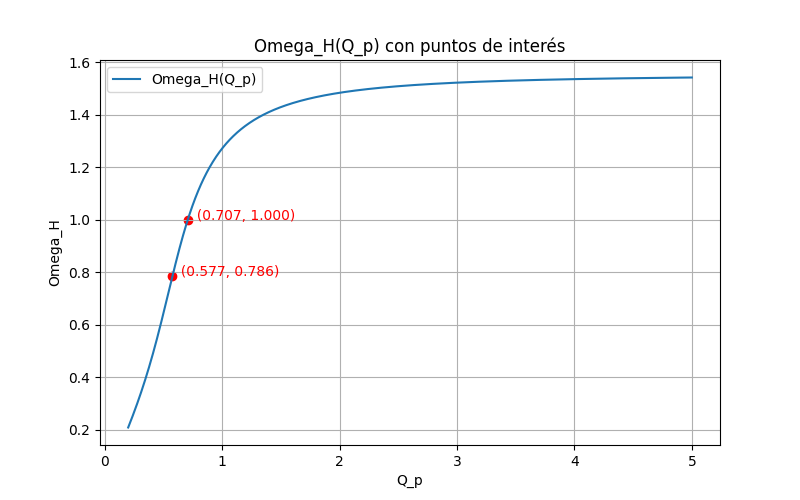
\includegraphics[width=1\textwidth]{Figura 1.png}
    \caption{Gráfica que define a $\Omega_{H}$ como función de $Q_{p}$} 
\end{figure}

Finalmente se añade la verificación numérica realizada en Python de los puntos de interés de esta gráfica:

\begin{figure}[H]
    \centering
    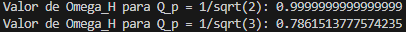
\includegraphics[width=0.7\textwidth]{Figura 2.png}
    \caption{Puntos de Interés según la Tabla (\ref{tab:tb_1}) de $Q_{p}$} 
\end{figure}



\subsection{Relación entre la Frecuencia Normalizada del Punto Crítico $(\Omega_{G})$ y el Factor de Calidad $(Q_{p})$}
La ecuación (\ref{eq_16}) desarrollada en el marco teórico, muestra la relación entre las variables de interés de esta sección. Desde esta ecuación despejaremos a $Q_{p}$ tal que:

\begin{equation}
    \label{eq_40}
    \Omega_G^4 + \frac{1}{Q_p^2} \Omega_G^2 - 1 = 0
\end{equation}

Si se define a $x=\Omega_G^2$ se tiene entonces que:

\begin{equation}
    \label{eq_41}
    x^2 + \left(\frac{1}{Q_p^2}\right)x - 1 = 0
\end{equation}

Nótese que se ha obtenido una expresión cuadrática para la cual, planteando la solución genérica de la misma, se tiene que:

\begin{equation}
    \label{eq_42}
    x_{1,2} = \frac{-\frac{1}{Q_{p}^{2}} \pm \sqrt{\left(\frac{1}{Q_{p}^{2}}\right)^{2} - 4(1)(-1)}}{2(1)}
\end{equation}

De aquí, se deduce que solo se busca la solución con frecuencia crítica normalizada positiva dada la inexistencia de frecuencias negativas, por lo tanto, se tiene que re acomodando algunos términos e incluyendo esta aclaración, se tiene que:

\begin{equation}
    \label{eq_43}
    x = \frac{-\frac{1}{Q_{p}^{2}} + \sqrt{\left(\frac{1}{Q_{p}^{2}}\right)^{2} + 4}}{2}
\end{equation}

Reemplazando a $x$ por $\Omega_{G}^{2}$, se deduce finalmente que:

\begin{equation}
    \label{eq_44}
    \Omega_{G} = \sqrt{\frac{-\frac{1}{Q_{p}^{2}} + \sqrt{\frac{1}{Q_{p}^{4}} + 4}}{2}}
\end{equation}

A continuación, se presenta una gráfica realizada en Python que muestra la relación obtenida en (\ref{eq_44}) tal que:

\begin{figure}[H]
    \centering
    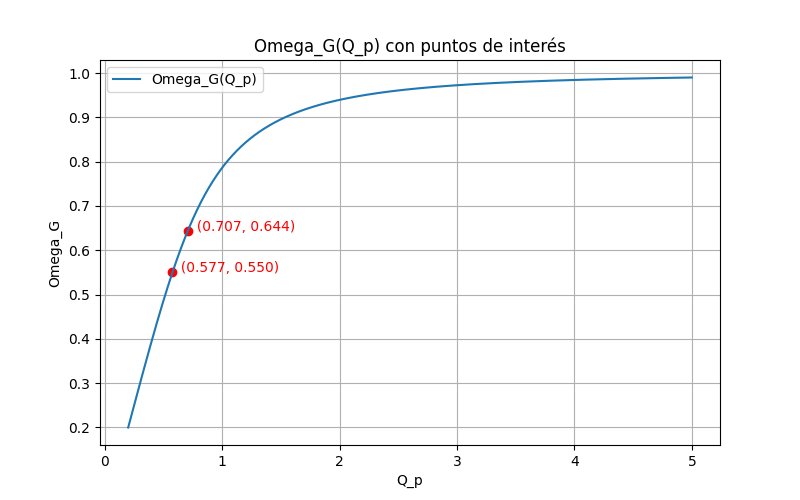
\includegraphics[width=1\textwidth]{Figura 3.png}
    \caption{Gráfica que define a $\Omega_{G}$ como función de $Q_{p}$} 
\end{figure}

Finalmente se añade la verificación numérica realizada en Python de los puntos de interés de esta gráfica:

\begin{figure}[H]
    \centering
    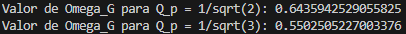
\includegraphics[width=0.7\textwidth]{Figura 4.png}
    \caption{Puntos de Interés según la Tabla (\ref{tab:tb_1}) de $Q_{p}$} 
\end{figure}



\subsection{Relación entre el Margen de Fase $(M\phi)$ y el Factor de Calidad $(Q_p)$}
El margen de fase expuesto tanto en (\ref{eq_19}) como en (\ref{eq_33}) tiene la particularidad que a diferencia de las 2 relaciones descritas anteriormente, es que esta no tan solo depende del factor de calidad $Q_{p}$ sino que también de la frecuencia crítica normalizada $\Omega_{G}$.

Para solventar este inconveniente, utilizaremos la expresión obtenida en (\ref{eq_44}) para poder definir a $\Omega_{G}$ en términos de $Q_{p}$. Por lo tanto, se plantea que partiendo ya sea de (\ref{eq_19}) como de (\ref{eq_33}), se tiene que:
\begin{equation}
    \label{eq_45}
    M\phi = \ang{90} - \arctan(\Omega_{G} Q_{p}) 
\end{equation}

Reemplazando $\Omega_{G}$ por la expresión obtenida en (\ref{eq_44}), resulta que:

\begin{equation}
    \label{eq_46}
    M\phi = \ang{90} - \arctan\left(\sqrt{\frac{-\frac{1}{Q_{p}^{2}} + \sqrt{\frac{1}{Q_{p}^{4}} + 4}}{2}} Q_{p}\right)
\end{equation}

A continuación, se presenta una gráfica realizada en Python que muestra la relación obtenida en (\ref{eq_46}) tal que:

\begin{figure}[H]
    \centering
    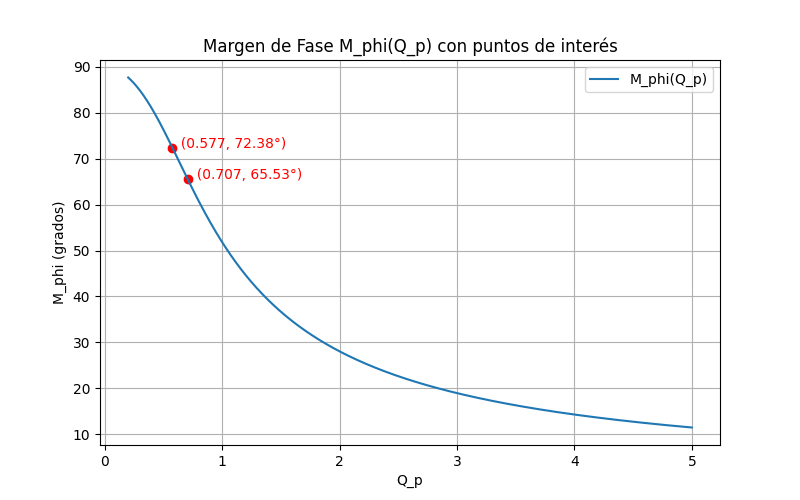
\includegraphics[width=0.9\textwidth]{Figura 5.png}
    \caption{Gráfica que define a $M\phi$ como función de $Q_{p}$} 
\end{figure}

Finalmente se añade la verificación numérica realizada en Python de los puntos de interés de esta gráfica:

\begin{figure}[H]
    \centering
    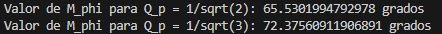
\includegraphics[width=0.7\textwidth]{Figura 6.png}
    \caption{Puntos de Interés según la Tabla (\ref{tab:tb_1}) de $Q_{p}$} 
\end{figure}
\\


\section{Conclusión}
En este informe, se ha demostrado como obtener los distintos gráficos que muestran las variaciones de distintas variables de interés para un amplificador, tales como: $\Omega_{H}$, $\Omega_{G}$ y $M\phi$ en función del factor de calidad $Q_{p}$ del mismo. Para ello se hizo extenso uso de la aritmética y el marco teórico presentado por el Dr. Ing. Pablo Ferreyra en su material de estudio para la asignatura de Síntesis de Redes Activas y así mismo como del lenguaje de programación de Python para realizar tanto las gráficas como las verificaciones numéricas para los puntos de interés de presentados en el cuadro (\ref{tab:tb_1}).
\\


\section{Bibliografía}
\begin{itemize}
    \item \href{https://fcefyn.aulavirtual.unc.edu.ar/pluginfile.php/959870/mod_resource/content/1/SRA-CapVI-VII_2013-Rev1.pdf}{Unidad VI - "Síntesis del Amplificador Compensado"}
    \item \href{https://github.com/ErnestMonja/Sintesis_de_Redes_Activas/tree/main}{Repositorio de GitHub con los códigos y demás archivos de este informe}
\end{itemize}
\\


\section{Anexo}
En este apartado se presentan los códigos de Python utilizados para realizar tanto las gráficas como los cálculos numéricos presentados en las figuras de este informe:

\begin{itemize}

\item \underline{Código para obtener a $\Omega_H$ en función de $Q_p$:}
\begin{minted}[linenos]{python}
import matplotlib
matplotlib.use("Qt5Agg")
    
import numpy as np
import matplotlib.pyplot as plt
    
# Defino a Omega_H como función de Q_p
def Omega_H(Qp):
    termino = (2 - 1/Qp**2 + np.sqrt((1/Qp**2 - 2)**2 + 4)) / 2
    return np.sqrt(termino)
    
# Defino el dominio que quiero graficar
Qp = np.linspace(0.2, 5, 1000)
Omega_vals = Omega_H(Qp)
    
# Defino y calculo los dos puntos de interes para Q_p
Qp1 = 1 / np.sqrt(2)
Qp2 = 1 / np.sqrt(3)
    
Omega1 = Omega_H(Qp1)
Omega2 = Omega_H(Qp2)
    
print("Valor de Omega_H para Q_p = 1/sqrt(2):", Omega1)
print("Valor de Omega_H para Q_p = 1/sqrt(3):", Omega2)
    
# Grafico
plt.figure(figsize=(8,5))
plt.plot(Qp, Omega_vals, label="Omega_H(Q_p)")
    
# Marco puntos
plt.scatter([Qp1, Qp2], [Omega1, Omega2], color='red')
plt.text(Qp1, Omega1, f"  ({Qp1:.3f}, {Omega1:.3f})", color='red')
plt.text(Qp2, Omega2, f"  ({Qp2:.3f}, {Omega2:.3f})", color='red')
    
plt.xlabel("Q_p")
plt.ylabel("Omega_H")
plt.title("Omega_H(Q_p) con puntos de interés")
plt.grid(True)
plt.legend()
plt.show()
\end{minted}

\item \underline{Código para obtener a $\Omega_G$ en función de $Q_p$:}
\begin{minted}[linenos]{python}
import matplotlib
matplotlib.use("Qt5Agg")
        
import numpy as np
import matplotlib.pyplot as plt
        
# Defino a Omega_G como función de Q_p
def Omega_G(Qp):
    termino = (- 1/Qp**2 + np.sqrt((1/Qp**2)**2 + 4)) / 2
    return np.sqrt(termino)
        
# Defino el dominio que quiero graficar
Qp = np.linspace(0.2, 5, 1000)
Omega_vals = Omega_G(Qp)
        
# Defino y calculo los dos puntos de interes para Q_p
Qp1 = 1 / np.sqrt(2)
Qp2 = 1 / np.sqrt(3)
        
Omega1 = Omega_G(Qp1)
Omega2 = Omega_G(Qp2)
        
print("Valor de Omega_G para Q_p = 1/sqrt(2):", Omega1)
print("Valor de Omega_G para Q_p = 1/sqrt(3):", Omega2)
        
# Grafico
plt.figure(figsize=(8,5))
plt.plot(Qp, Omega_vals, label="Omega_G(Q_p)")
        
# Marco puntos
plt.scatter([Qp1, Qp2], [Omega1, Omega2], color='red')
plt.text(Qp1, Omega1, f"  ({Qp1:.3f}, {Omega1:.3f})", color='red')
plt.text(Qp2, Omega2, f"  ({Qp2:.3f}, {Omega2:.3f})", color='red')
        
plt.xlabel("Q_p")
plt.ylabel("Omega_G")
plt.title("Omega_G(Q_p) con puntos de interés")
plt.grid(True)
plt.legend()
plt.show()
\end{minted}

\item \underline{Código para obtener a $M\phi$ en función de $Q_p$:}
\begin{minted}[linenos]{python}
import matplotlib
matplotlib.use("Qt5Agg")

import numpy as np
import matplotlib.pyplot as plt

# Defino ahora a M-phi como función de y Q_p
def M_phi(Qp):
    # Parte interna de la raíz
    termino = (-1/Qp**2 + np.sqrt((1/Qp**2)**2 + 4)) / 2
    dentro = Qp * np.sqrt(termino)

    # M_phi en grados
    return 90 - np.degrees(np.arctan(dentro))

# Defino el dominio que quiero graficar
Qp = np.linspace(0.2, 5, 1000)
M_vals = M_phi(Qp)

# Defino y calculo los dos puntos de interes para Q_p
Qp1 = 1 / np.sqrt(2)
Qp2 = 1 / np.sqrt(3)

M1 = M_phi(Qp1)
M2 = M_phi(Qp2)

print("Valor de M_phi para Q_p = 1/sqrt(2):", M1, "grados")
print("Valor de M_phi para Q_p = 1/sqrt(3):", M2, "grados")

# Grafico
plt.figure(figsize=(8,5))
plt.plot(Qp, M_vals, label="M_phi(Q_p)")

# Marco puntos
plt.scatter([Qp1, Qp2], [M1, M2], color='red')
plt.text(Qp1, M1, f"  ({Qp1:.3f}, {M1:.2f}°)", color='red')
plt.text(Qp2, M2, f"  ({Qp2:.3f}, {M2:.2f}°)", color='red')

plt.xlabel("Q_p")
plt.ylabel("M_phi (grados)")
plt.title("Margen de Fase M_phi(Q_p) con puntos de interés")
plt.grid(True)
plt.legend()
plt.show()
\end{minted}
\end{itemize}
    


\end{document}
